\chapter{Components}

In this chapter, all relevant parts of the system are explained and reasons are given why they were selected.

\section{Touch Screen}

    

\section{Main Controller}

    For the Main Controller the Raspberry Pi ??? was choosen as it provides enough computaional power to handle the input from the touch screen, host the database, and communicate with the Micro Controller. In addition it comes with a connection to the display and enough USB-A Connections to connect to all three microcontrollers.

\section{Database}



    \begin{figure}[h]
        \centering
        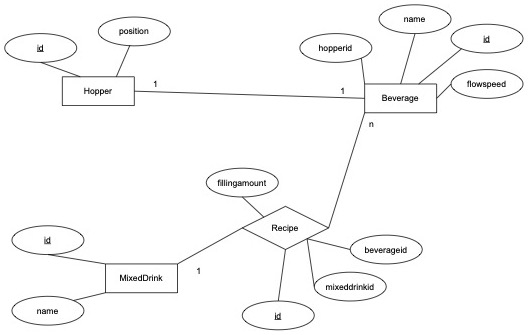
\includegraphics[width=120mm]{content/figures/database.jpg}
        \caption{Database structure \label{fig:database}}
    \end{figure}


\section{Micro Controller}

    For the microcontrollers, the choice fell on the  \textit{RP2040} \cite{rp2040}. With the help of the \textit{Raspberry Pi Pico SDK} \cite{sdk} it is relatively easy to write programs in the C language for it. The peripherals include 2 UARTs for easy communication with the stepper drivers. 

    The controllers were used in the form of the \textit{Tiny 2040} \cite{tiny2040}. The \textit{Tiny 2040} is a development board that complements the \textit{RP2040} with a USB-C connector and easily accessible IO pins.


\section{Stepper driver}

    \textit{TMC2209s} were selected as stepper drivers because they offer a UART interface that provides reliable communication and allows a wide range of settings. 
    Up to four drivers can be connected simultaneously to one UART master. In addition, they operate almost silently. \cite{tmc2209}

    For communication with the stepper drivers, a \textit{TMC2209} library \cite{tmcLibrary} and a \textit{Serial-over-UART} implementation, both originally written for the \textit{Arduion IDE} in \textit{C++}, were rewritten in \textit{C}.

\section{Mototor}



\section{Limit Switch}

    A limit switch lets current through when it is closed and not when it is open. Therefore, it can be detected when a specified physical limit is reached.

\section{LED}



\section{Power Supply}


